\documentclass[11pt, a4paper]{article}
\usepackage{pdfpages}
\usepackage{parallel}
\usepackage[T2A]{fontenc}
\usepackage{ucs}
\usepackage[utf8x]{inputenc}
\usepackage[polish,english,russian]{babel}
\usepackage{hyperref}
\usepackage{rotating}
\usepackage[inner=2cm,top=1.8cm,outer=2cm,bottom=2.3cm,nohead]{geometry}
\usepackage{listings}
\usepackage{graphicx}
\usepackage{wrapfig}
\usepackage{longtable}
\usepackage{indentfirst}
\usepackage{array}
\usepackage{tikzsymbols}
\usepackage{soul}
\usepackage[ruled,vlined]{algorithm2e}
%\counterwithout{figure}{section} 

\usepackage{url}
\makeatletter
\g@addto@macro{\UrlBreaks}{\UrlOrds}
\makeatother

\newcolumntype{P}[1]{>{\raggedright\arraybackslash}p{#1}}
\frenchspacing
\usepackage{fixltx2e} %text sub- and superscripts
\usepackage{icomma} % коскі ў матэматычным рэжыме
\PreloadUnicodePage{4}

\newcommand{\longpage}{\enlargethispage{\baselineskip}}
\newcommand{\shortpage}{\enlargethispage{-\baselineskip}}

\def\switchlang#1{\expandafter\csname switchlang#1\endcsname}
\def\switchlangbe{
\let\saverefname=\refname%
\def\refname{Літаратура}%
\def\figurename{Іл.}%
}
\def\switchlangen{
\let\saverefname=\refname%
\def\refname{References}%
\def\figurename{Fig.}%
}
\def\switchlangru{
\let\saverefname=\refname%
\let\savefigurename=\figurename%
\def\refname{Литература}%
\def\figurename{Рис.}%
}

\hyphenation{admi-ni-stra-tive}
\hyphenation{ex-pe-ri-ence}
\hyphenation{fle-xi-bi-li-ty}
\hyphenation{Py-thon}
\hyphenation{ma-the-ma-ti-cal}
\hyphenation{re-ported}
\hyphenation{imp-le-menta-tions}
\hyphenation{pro-vides}
\hyphenation{en-gi-neering}
\hyphenation{com-pa-ti-bi-li-ty}
\hyphenation{im-pos-sible}
\hyphenation{desk-top}
\hyphenation{elec-tro-nic}
\hyphenation{com-pa-ny}
\hyphenation{de-ve-lop-ment}
\hyphenation{de-ve-loping}
\hyphenation{de-ve-lop}
\hyphenation{da-ta-ba-se}
\hyphenation{plat-forms}
\hyphenation{or-ga-ni-za-tion}
\hyphenation{pro-gramming}
\hyphenation{in-stru-ments}
\hyphenation{Li-nux}
\hyphenation{sour-ce}
\hyphenation{en-vi-ron-ment}
\hyphenation{Te-le-pathy}
\hyphenation{Li-nux-ov-ka}
\hyphenation{Open-BSD}
\hyphenation{Free-BSD}
\hyphenation{men-ti-on-ed}
\hyphenation{app-li-ca-tion}

\def\progref!#1!{\texttt{#1}}
\renewcommand{\arraystretch}{2} %Іначай формулы ў матрыцы зліпаюцца з лініямі
\usepackage{array}

\def\interview #1 (#2), #3, #4, #5\par{

\section[#1, #3, #4]{#1 -- #3, #4}
\def\qname{LVEE}
\def\aname{#1}
\def\q ##1\par{{\noindent \bf \qname: ##1 }\par}
\def\a{{\noindent \bf \aname: } \def\qname{L}\def\aname{#2}}
}

\def\interview* #1 (#2), #3, #4, #5\par{

\section*{#1\\{\small\rm #3, #4. #5}}
\ifx\ParallelWhichBox\undefined%
    \addcontentsline{toc}{section}{#1, #3, #4}%
\else%
\ifnum\ParallelWhichBox=0%
    \addcontentsline{toc}{section}{#1, #3, #4}%
\fi\fi%

\def\qname{LVEE}
\def\aname{#1}
\def\q ##1\par{{\noindent \bf \qname: ##1 }\par}
\def\a{{\noindent \bf \aname: } \def\qname{L}\def\aname{#2}}
}

\newcommand{\interviewfooter}[1]{
\vskip 1em
\noindent \textit{#1}
}

\switchlang{en}
\begin{document}

\title{1996 "--- Kensington Expert Mouse Trackball 5.0}
\date{}
\maketitle
\selectlanguage{english}
In 1996, Kensington released its fifth Expert Mouse Trackball. The trackball has undergone a significant redesign \cite{KensingtonPC}. While previous models were fairly classic two-button devices, the Expert Mouse Trackball 5.0 is equipped with a larger diameter ball and four large buttons arranged symmetrically around the ball, similar to flower petals (figure \ref{fig:ExpertMousePic}).

\begin{figure}[h]
    \centering
    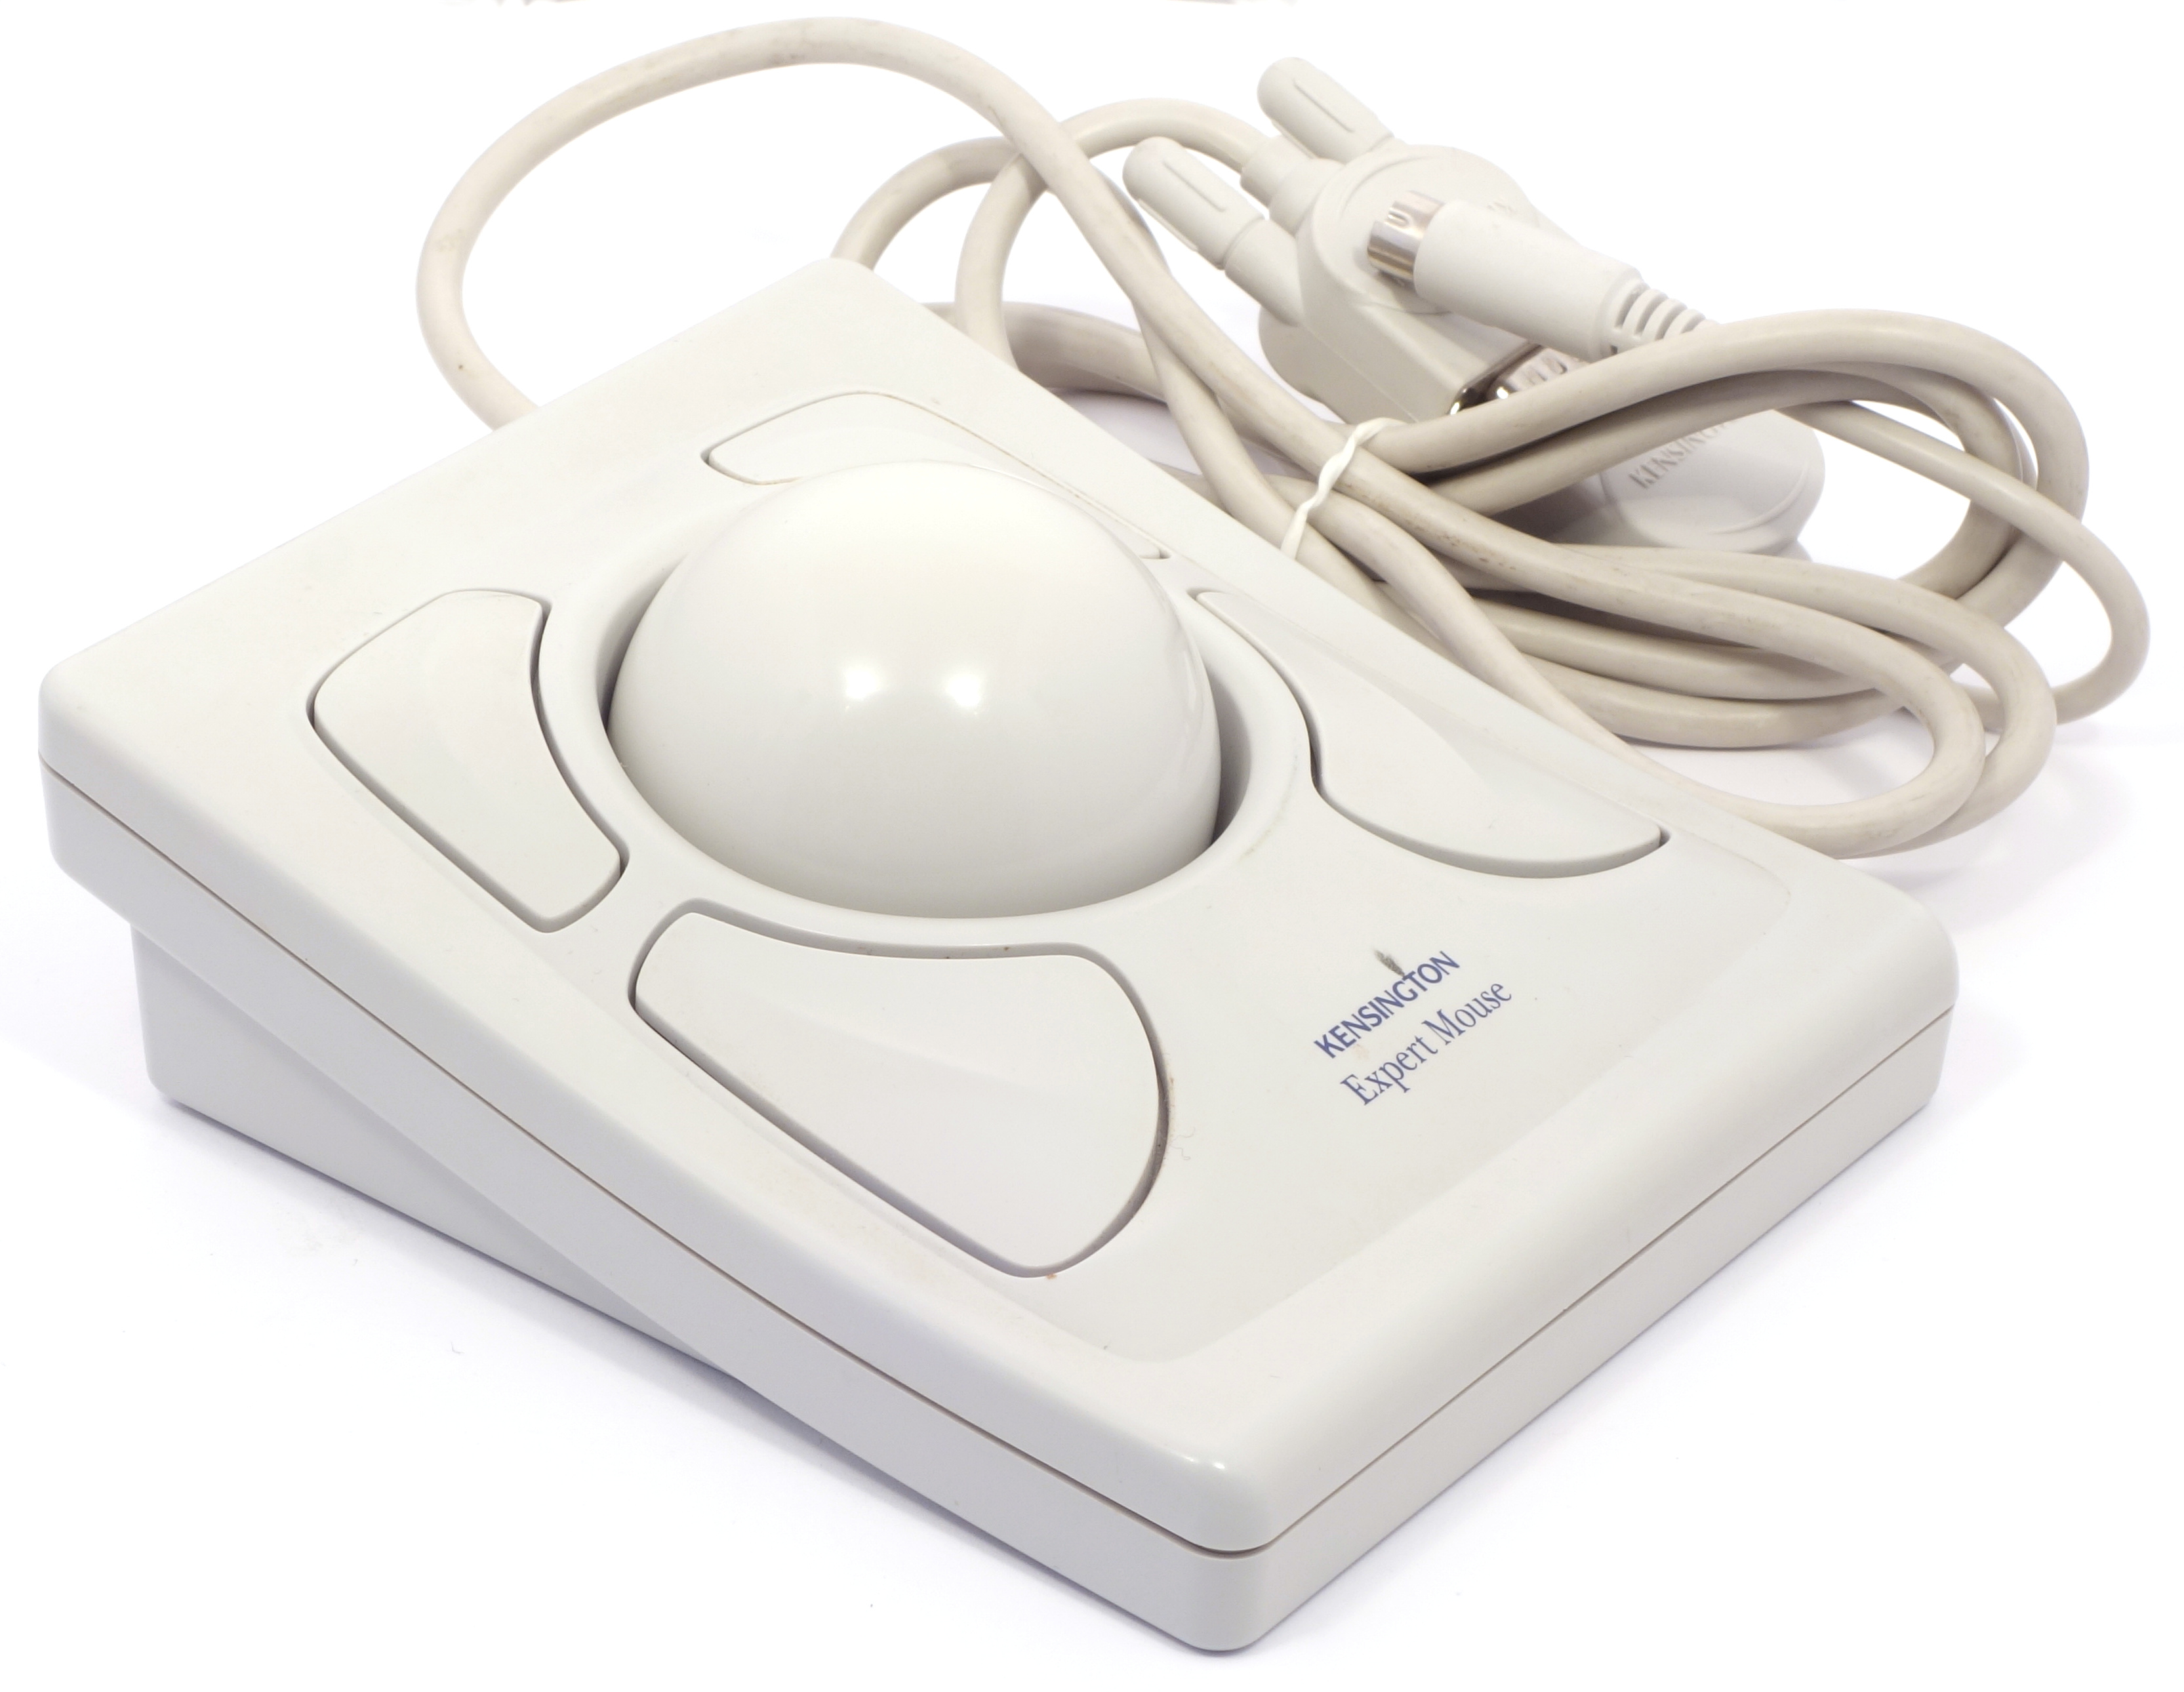
\includegraphics[scale=0.4]{1996_kensington_expert_trackball_5/pic_60.jpg}
    \caption{Kensington Expert Trackball}
    \label{fig:ExpertMousePic}
\end{figure}

A similar model was released for the Macintosh, which was predictably named Turbo Mouse 5.0 \cite{KensingtonMac} and equipped with an ADB interface, while the Expert Mouse was equipped with interchangeable cables for connecting to a serial interface and a PS / 2 port (and a bus version was also released separately with ISA adapter). Visually, Turmo Mouse and Expert Mouse were identical, reproducing the same “flowery” style (figure \ref{fig:ExpertMouseTopBottom}).

\begin{figure}[h]
    \centering
    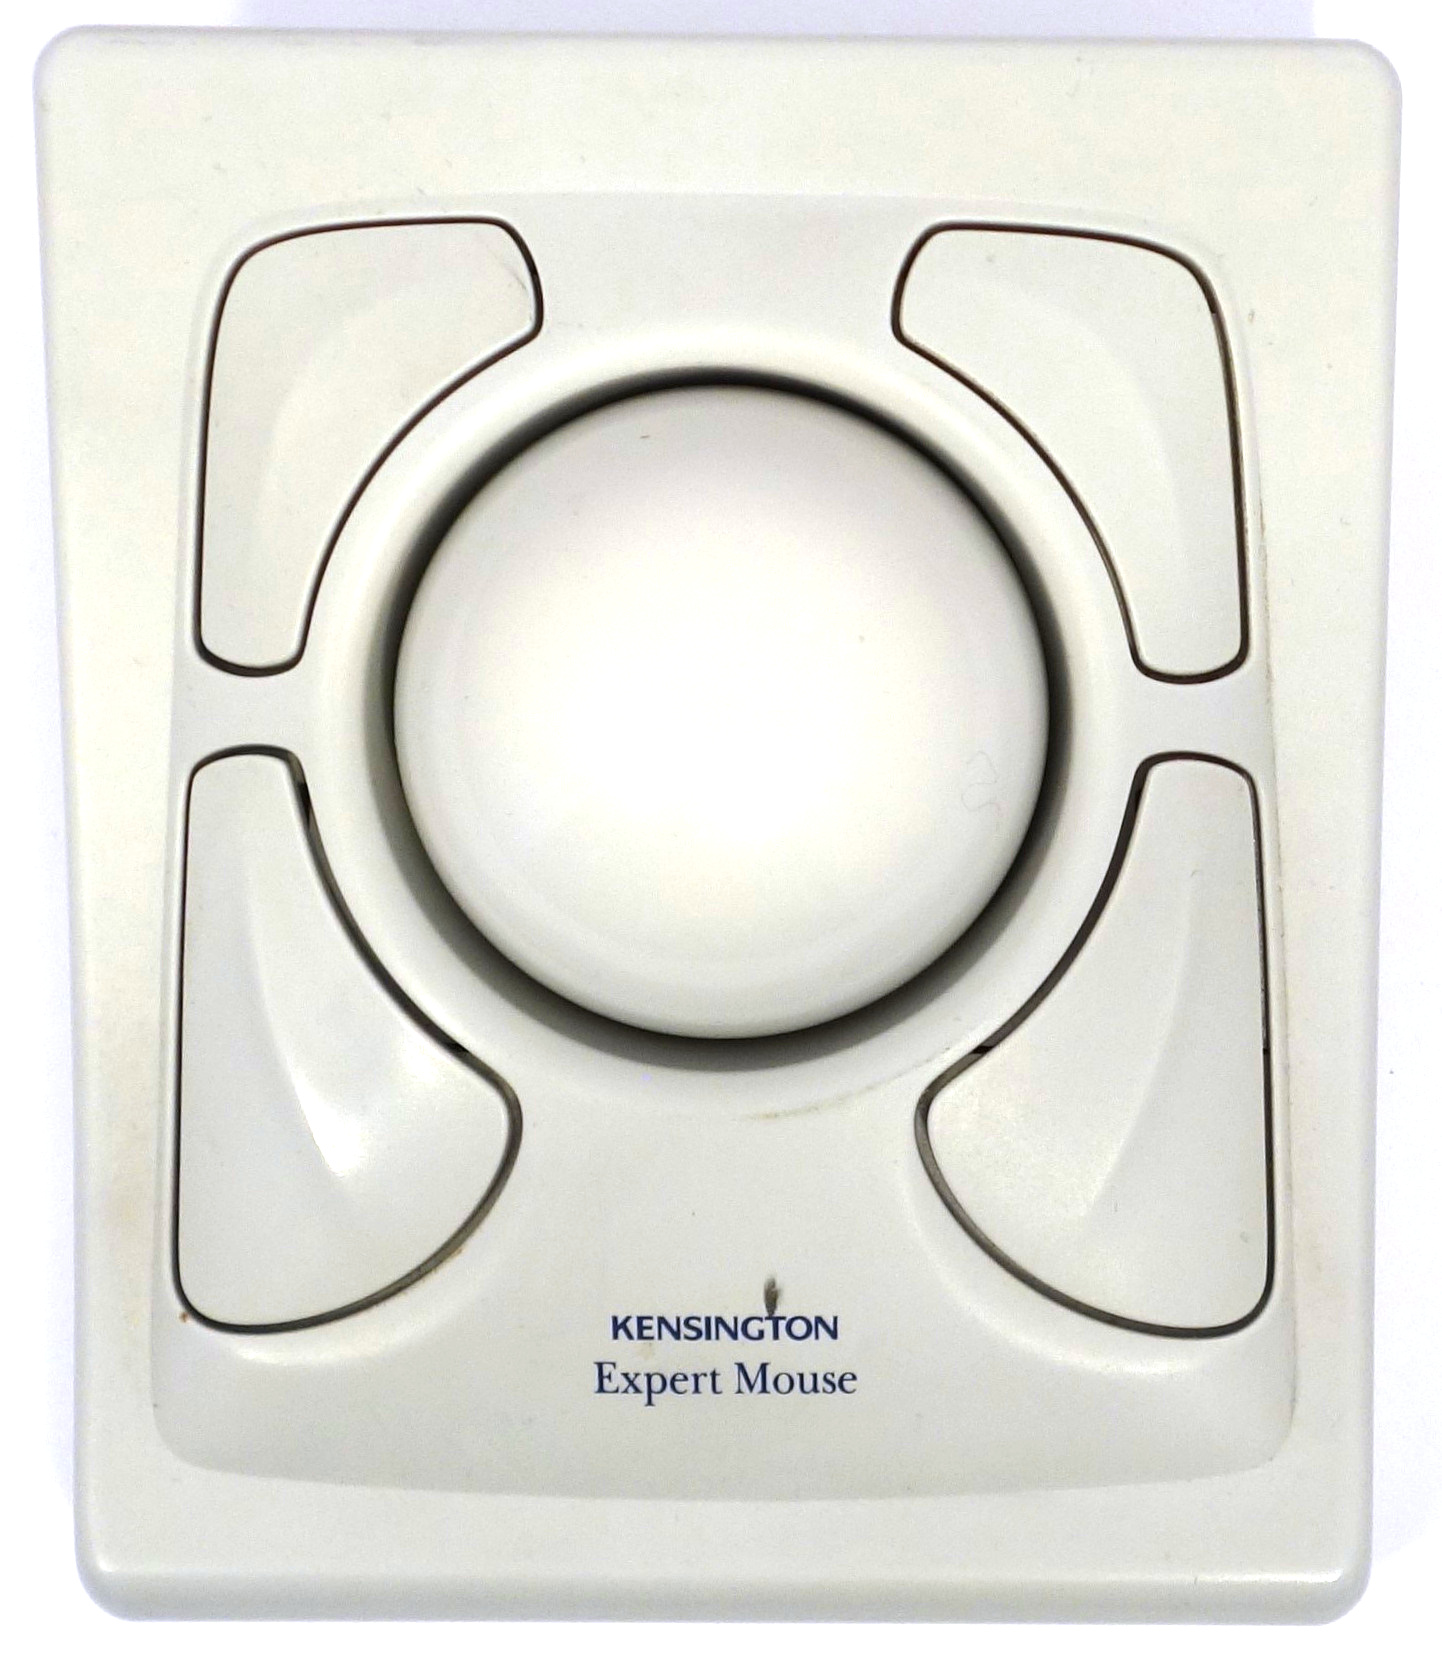
\includegraphics[scale=0.4]{1996_kensington_expert_trackball_5/top_30.jpg}
    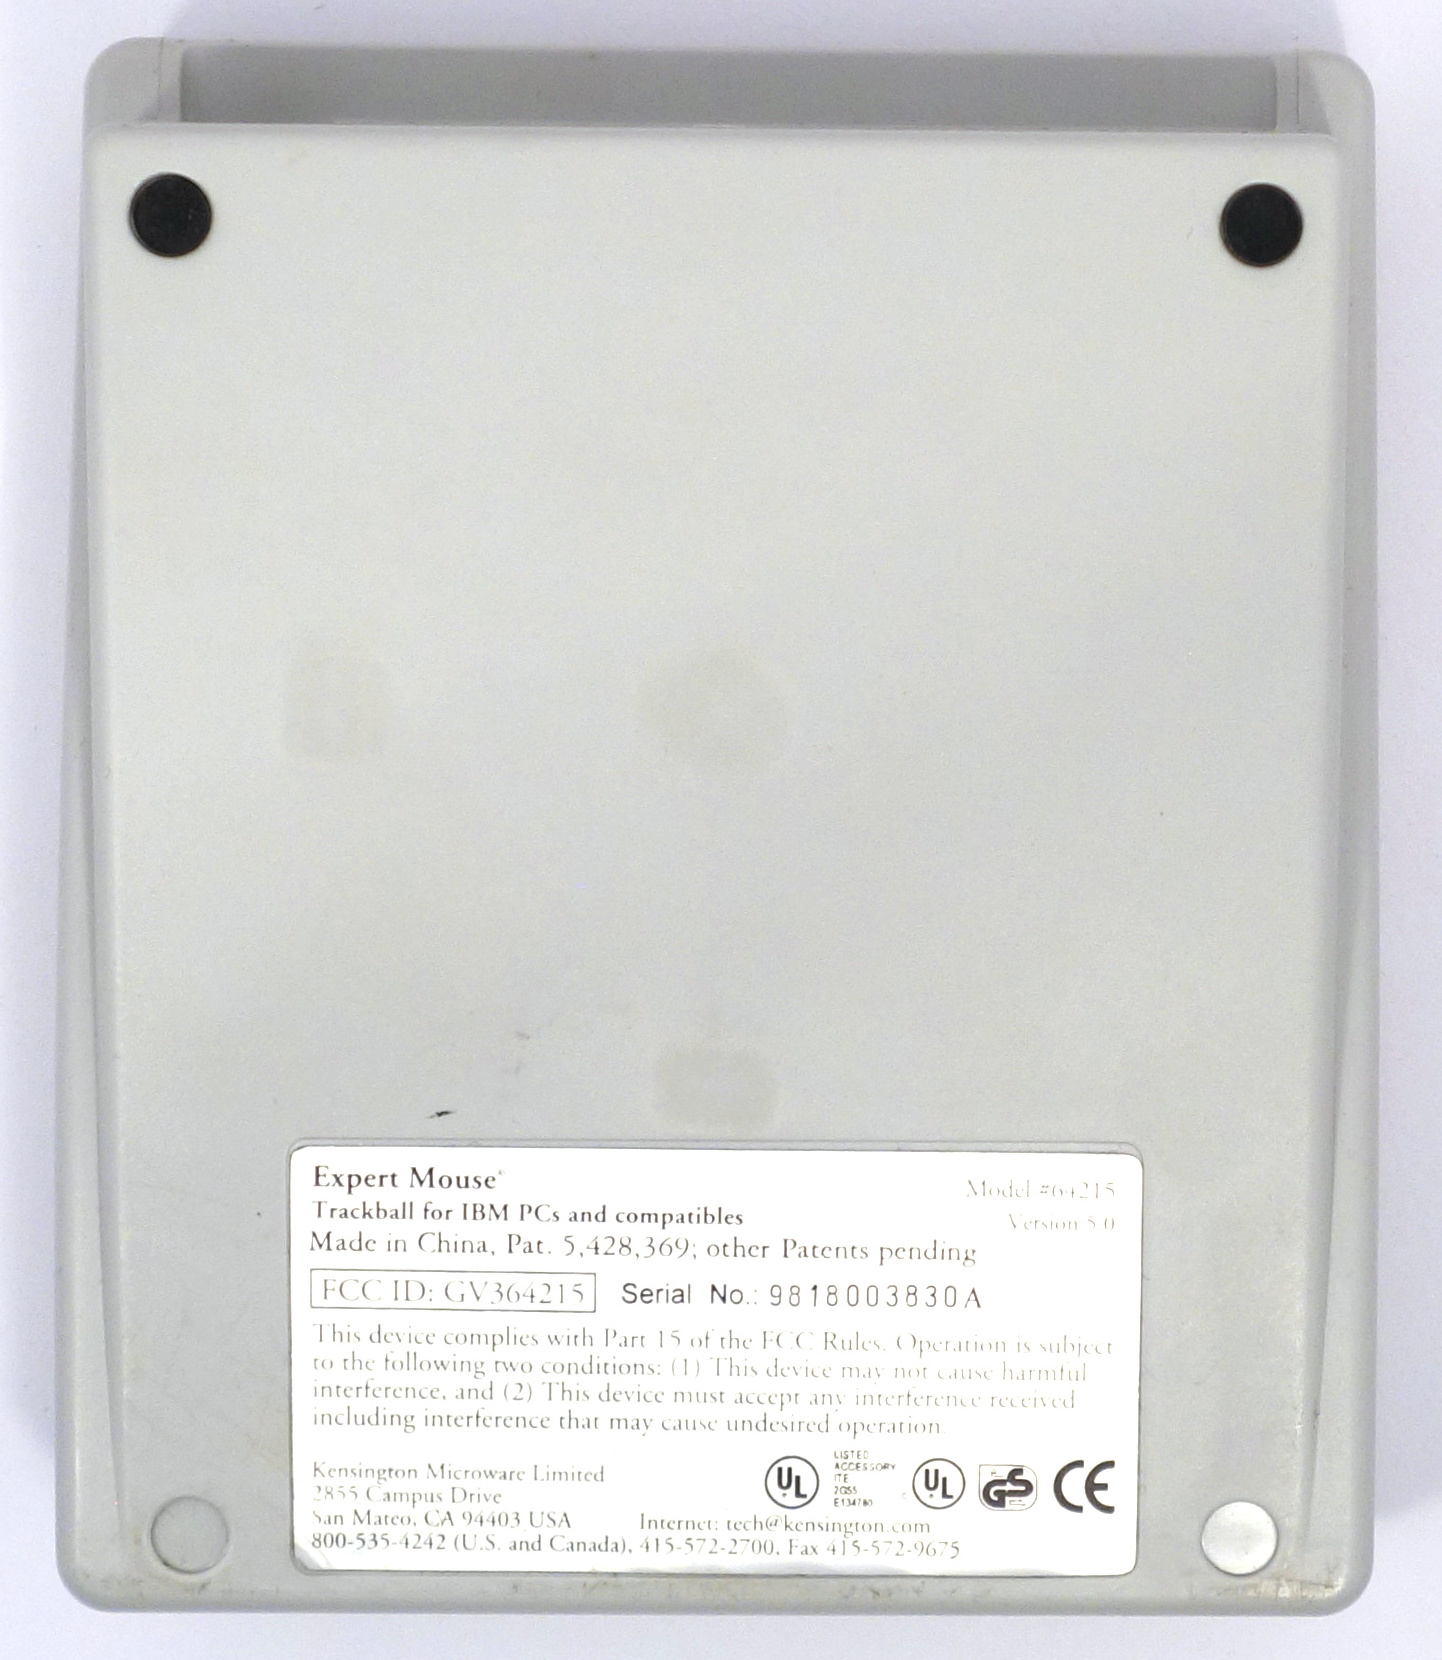
\includegraphics[scale=0.4]{1996_kensington_expert_trackball_5/bottom_30.jpg}
    \caption{Kensington Expert Mouse Trackball, top and bottom views}
    \label{fig:ExpertMouseTopBottom}
\end{figure}

Despite the large ball and large buttons, the Expert Mouse Trackball is not a very large device (figure \ref{fig:ExpertMouseSize}): in fact, the cavity for the ball and buttons takes up most of the body. It is also unusual that the ball is not fixed in any way and lies freely in a spherical cavity (therefore, in addition to floristic associations, the position of the ball also suggests an egg in a bird's nest). This greatly facilitates the cleaning of the device (but makes it difficult to carry it from place to place, since tilting the body from a horizontal position when carrying means dropping the ball on the floor).

\begin{figure}[h]
    \centering
    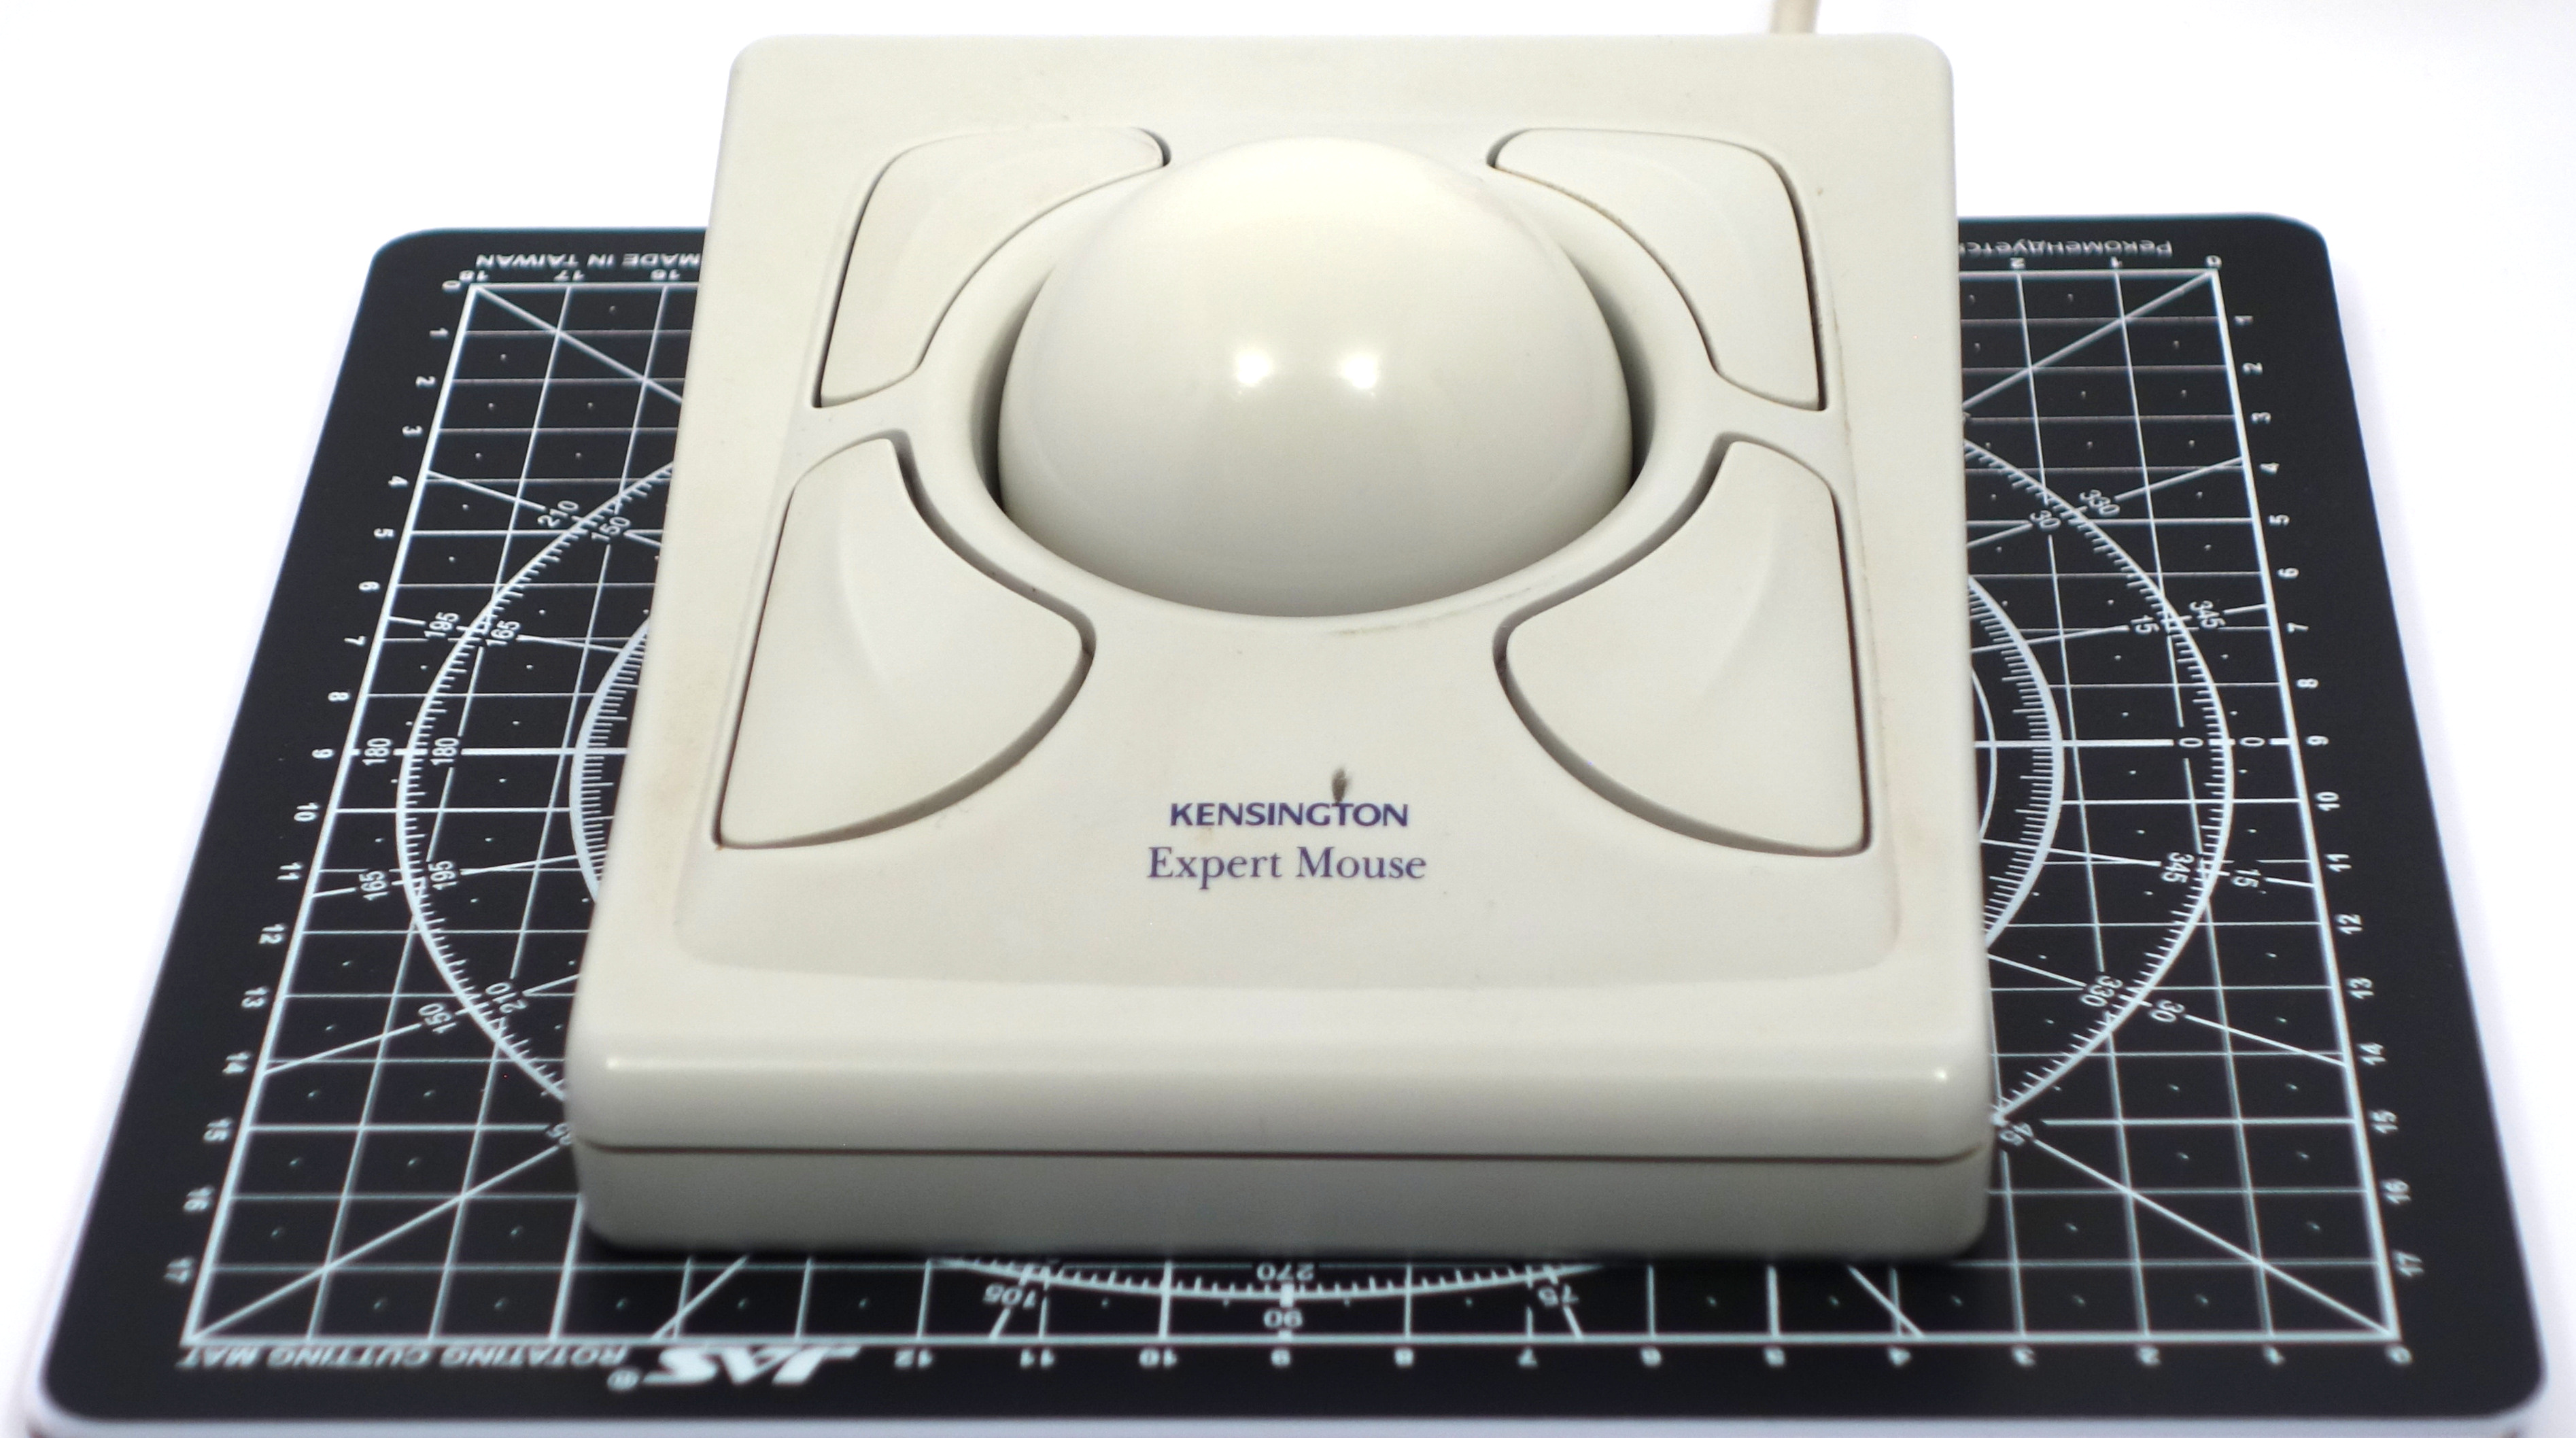
\includegraphics[scale=0.3]{1996_kensington_expert_trackball_5/size_30.jpg}
    \caption{Kensington Expert Mouse Trackball on a graduated pad with a grid step of 1~cm}
    \label{fig:ExpertMouseSize}
\end{figure}

Of course, a ball of this diameter is designed for precision cursor movement, which is in demand in CAD systems and graphic editors (given the non-standard design concept, it can be assumed that the calculation was made largely for this last category). In terms of ergonomics, the unusual arrangement of the buttons turns out to be quite convenient: during operation, the user covers the ball with his fingers and, depending on the position of the hand, is able to reach either two near or one near and two far buttons without moving his hand (figure \ref{fig:ExpertMouseHand}). By default, the two buttons closest to the user (and having the largest size) play the role of the left and right mouse buttons, which certainly simplifies the work for those who do not need additional buttons or rarely need them. A positive characteristic of the device's ergonomics is the symmetry of the case, typical for Kensington, which makes the device equally convenient for both left-handers and right-handers.

\begin{figure}[h]
    \centering
    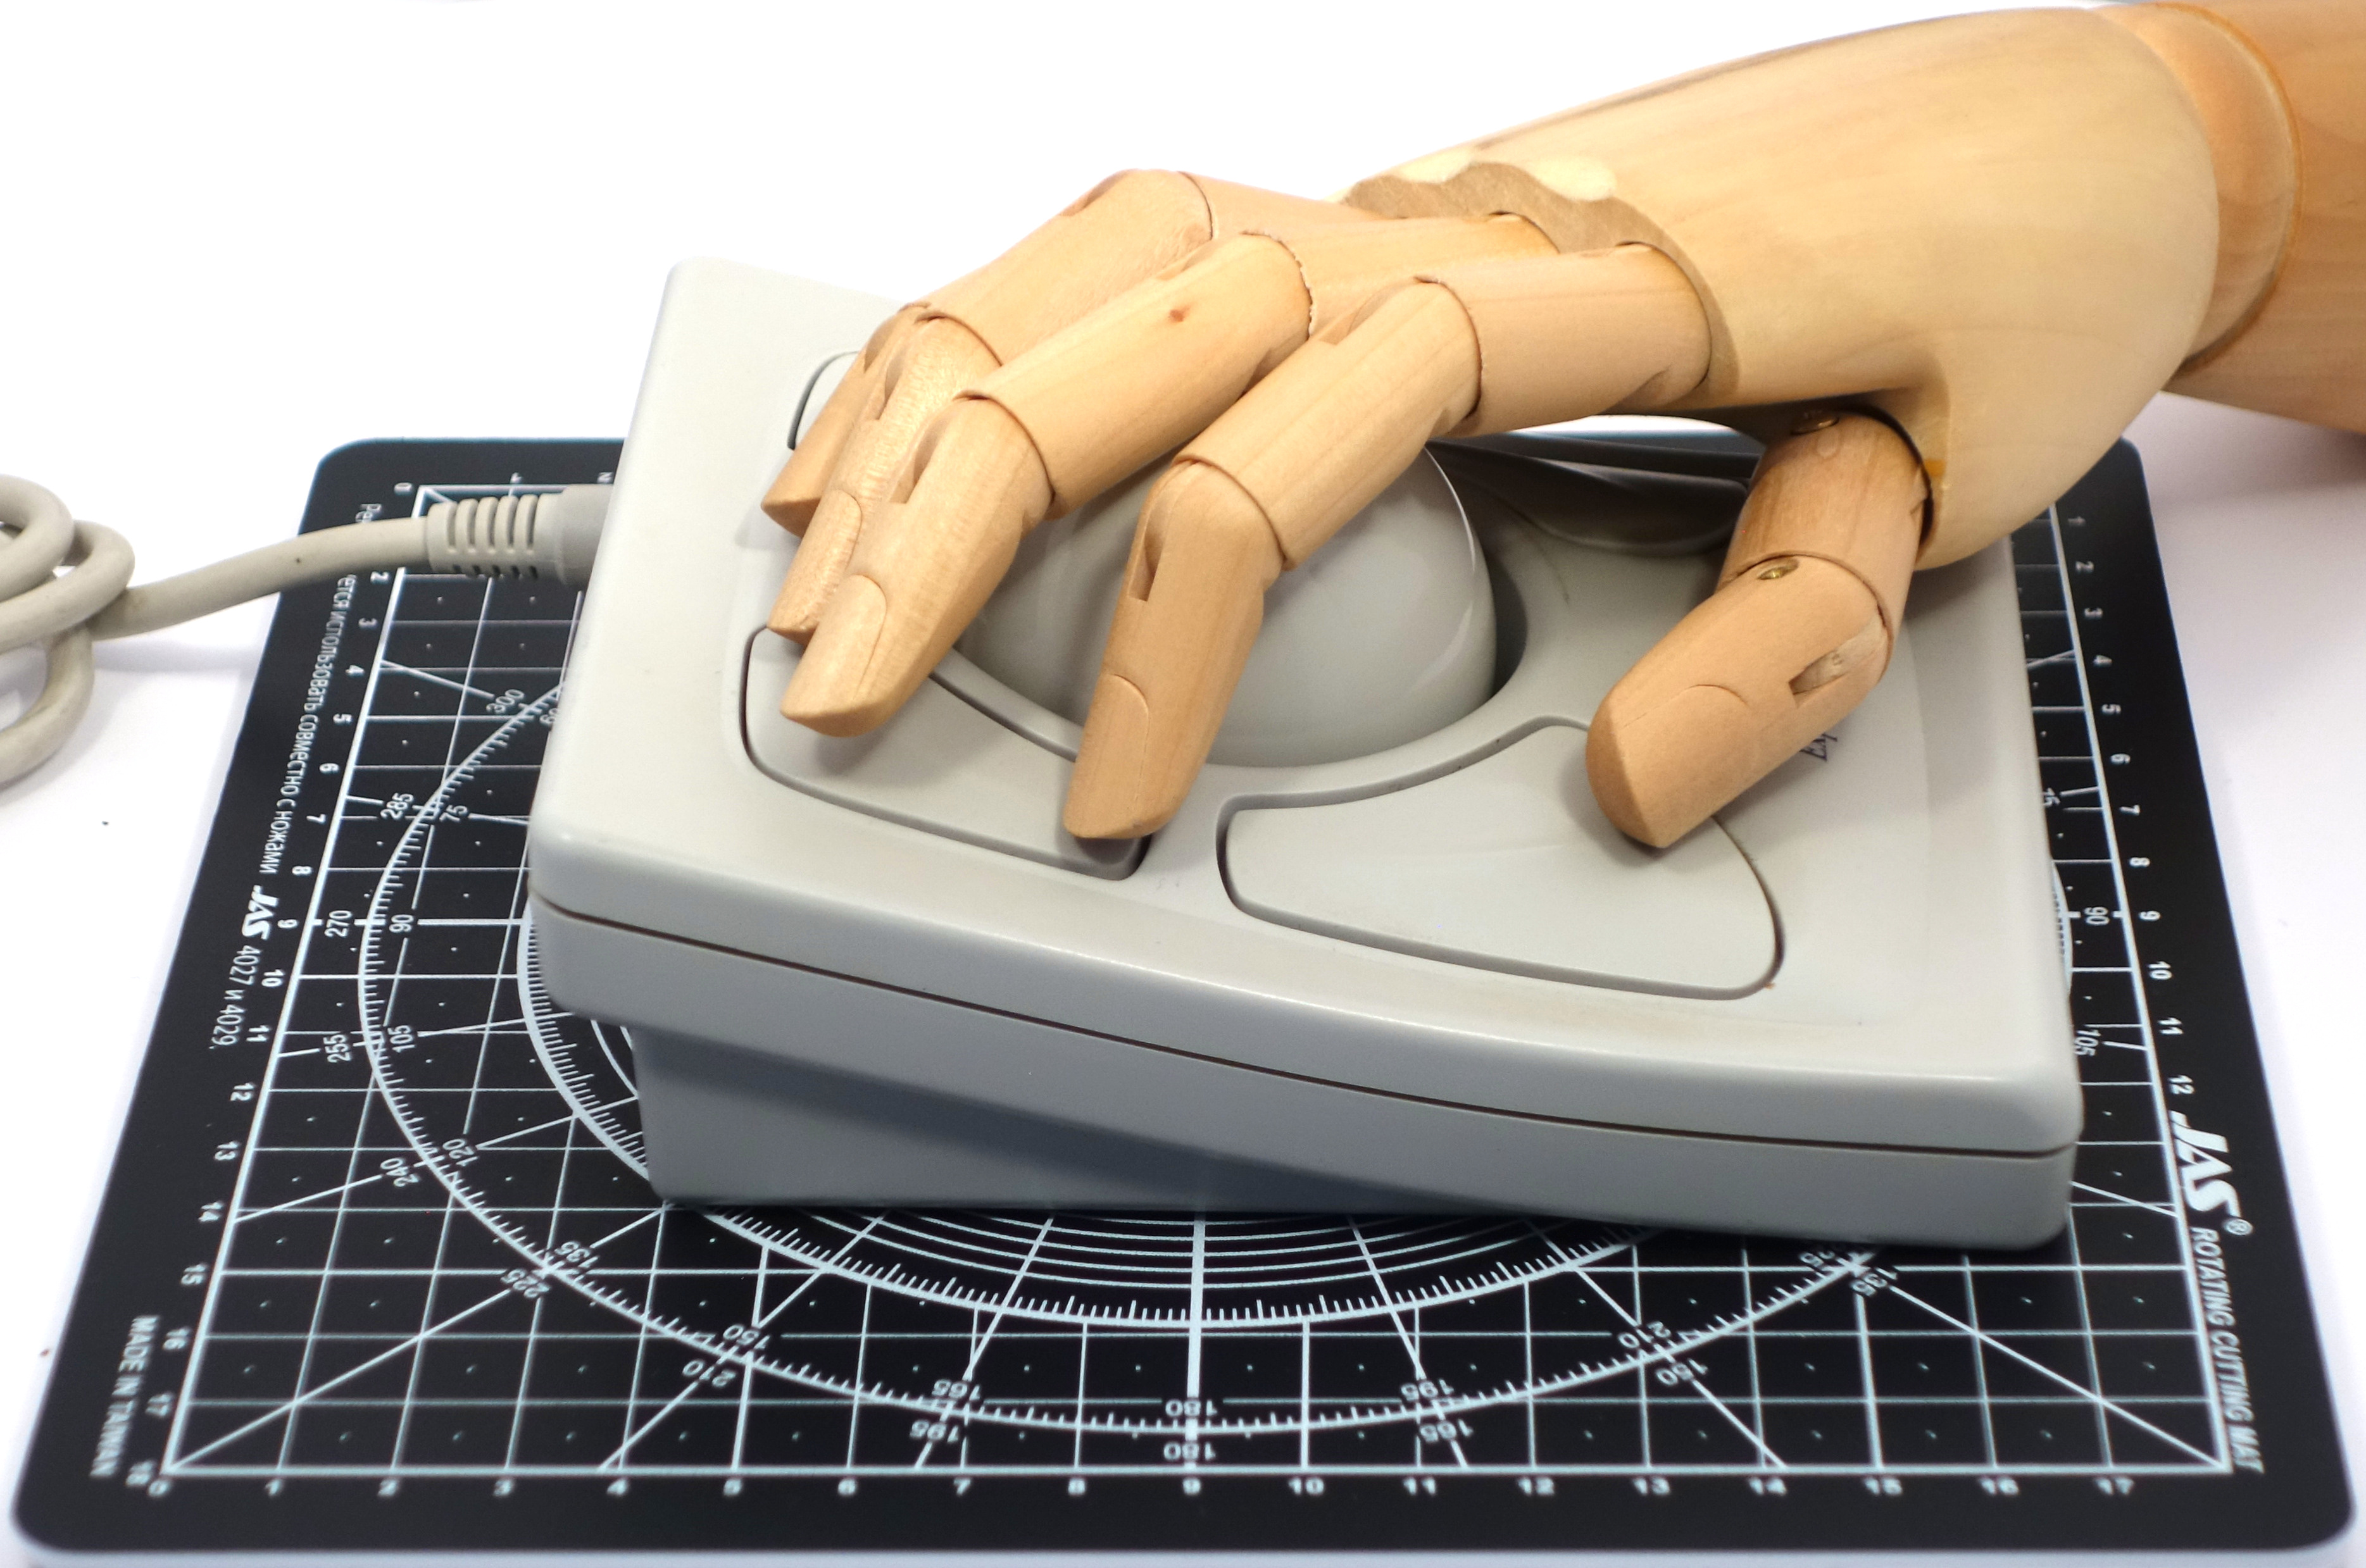
\includegraphics[scale=0.3]{1996_kensington_expert_trackball_5/hand_30.jpg}
    \caption{Kensington Expert Mouse Trackball with a human hand model}
    \label{fig:ExpertMouseHand}
\end{figure}

Trackball internals are shown on figure \ref{fig:ExpertMouseInside}. The standard opto-mechanical design is supplemented by durable massive metal rollers. At the same time, the optomechanical transformation is non-standard, it is made according to the patented “optical lever”  technology \cite{eu}. Instead of detecting light, which has passed through the slots of the rotating disk (as in most optmichanic trackballs and mice), a reflection of light from the radial metal “ribs” located on the end of the roller is detected - in fact, these are the ribs on the side of the bearing, driven by the rotation of the ball. Obviously, the high density of the ribs allowed the developers to abandon the disk, thereby reducing the dimensions of the device without reducing the resolution.

\begin{figure}[h]
    \centering
    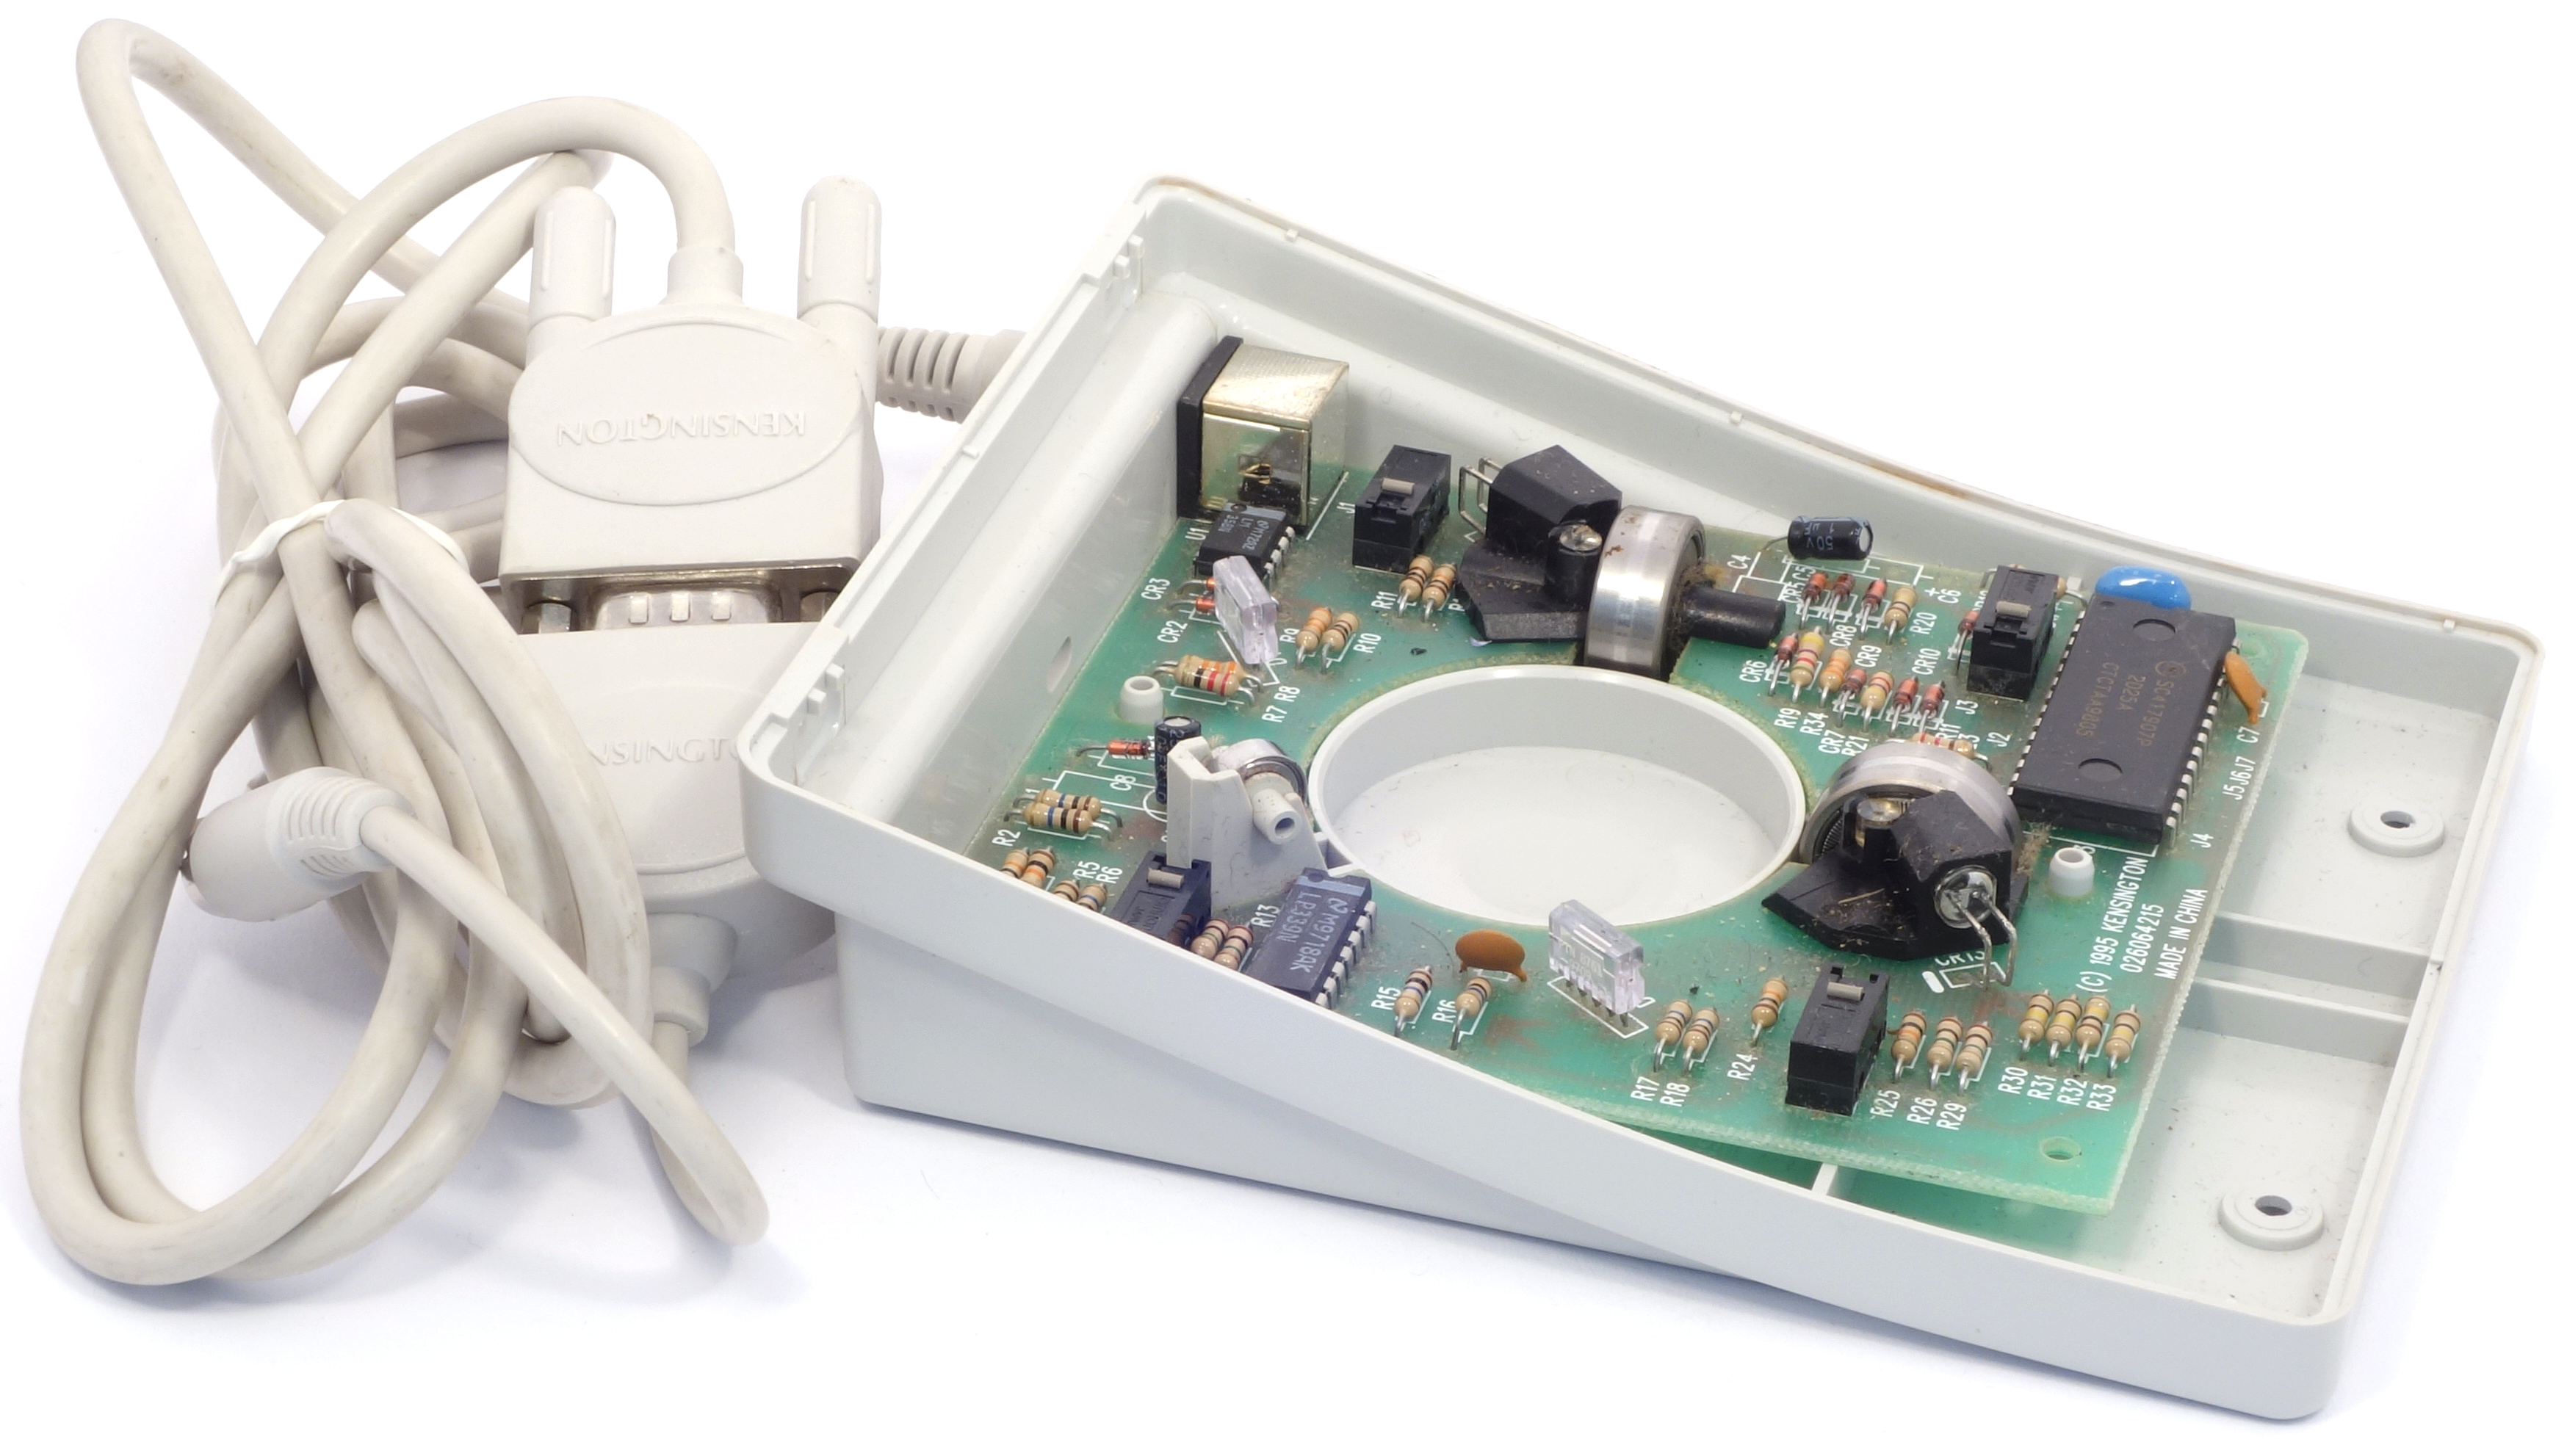
\includegraphics[scale=0.65]{1996_kensington_expert_trackball_5/inside_60.jpg}
    \caption{Kensington Expert Mouse Trackball disassembled}
    \label{fig:ExpertMouseInside}
\end{figure}

\begin{thebibliography}{9}

\bibitem {KensingtonPC} Kensington: Expert Mouse 5.0 "--- \url{https://web.archive.org/web/19970106170305/http://www.kensington.com/prod/mice/mice3b.html}
\bibitem {KensingtonMac} Kensington: Turbo Mouse 5.0 "--- \url{https://web.archive.org/web/19970106170317/http://www.kensington.com/prod/mice/mice3a.html}
\bibitem {eu} Kensington -- Trackballs.EU "--- \url{https://web.archive.org/web/20210423041707/https://forum.trackballs.eu/viewtopic.php?f=14&t=43}
\end{thebibliography}

\end{document}
